\documentclass[12pt]{report}
\usepackage[utf8]{inputenc}
\usepackage{cite}
\usepackage[hidelinks]{hyperref}
\usepackage{graphicx}
\usepackage{amsfonts}
\usepackage{mathtools}
\usepackage{caption}
\usepackage{fancyhdr}

\pagestyle{fancy}
\fancyhf{}
\rhead{5-stage Pipelined Processor Design Report}
\lhead{\thesection}
\rfoot{\thepage}

\DeclarePairedDelimiter\ceil{\lceil}{\rceil}
\DeclarePairedDelimiter\floor{\lfloor}{\rfloor}

\title{\textbf{5-stage Pipelined Processor Design Report}\\Team \#4}
\author{
  Mohamed Shawky\\
  \small\texttt{SEC:2, BN:16}
  \and
  Remonda Talaat\\
  \small\texttt{SEC:1, BN:20}
  \and
  Evram Youssef\\
  \small\texttt{SEC:1, BN:9}
  \and
  Mahmoud Adas\\
  \small\texttt{SEC:2, BN:21}
}
\date{\today}

\begin{document}

\thispagestyle{empty}

\maketitle
\tableofcontents
\listoffigures
\listoftables
\clearpage

\pagenumbering{arabic}

\part{Introduction}

\section{System Overview}
This document reports our design work of the 5-stage pipelined processor using Harvard
architecture. We discuss the overall system blocks and connections, the functionalities of the
different blocks and the hazard solutions. 

\section{Task Distribution}
\textbf{TODO: Task distribution table}

\part{Overall System}

\section{Overall System Design Schema}
\begin{center}
    \begin{figure}[hp]
        \centering
        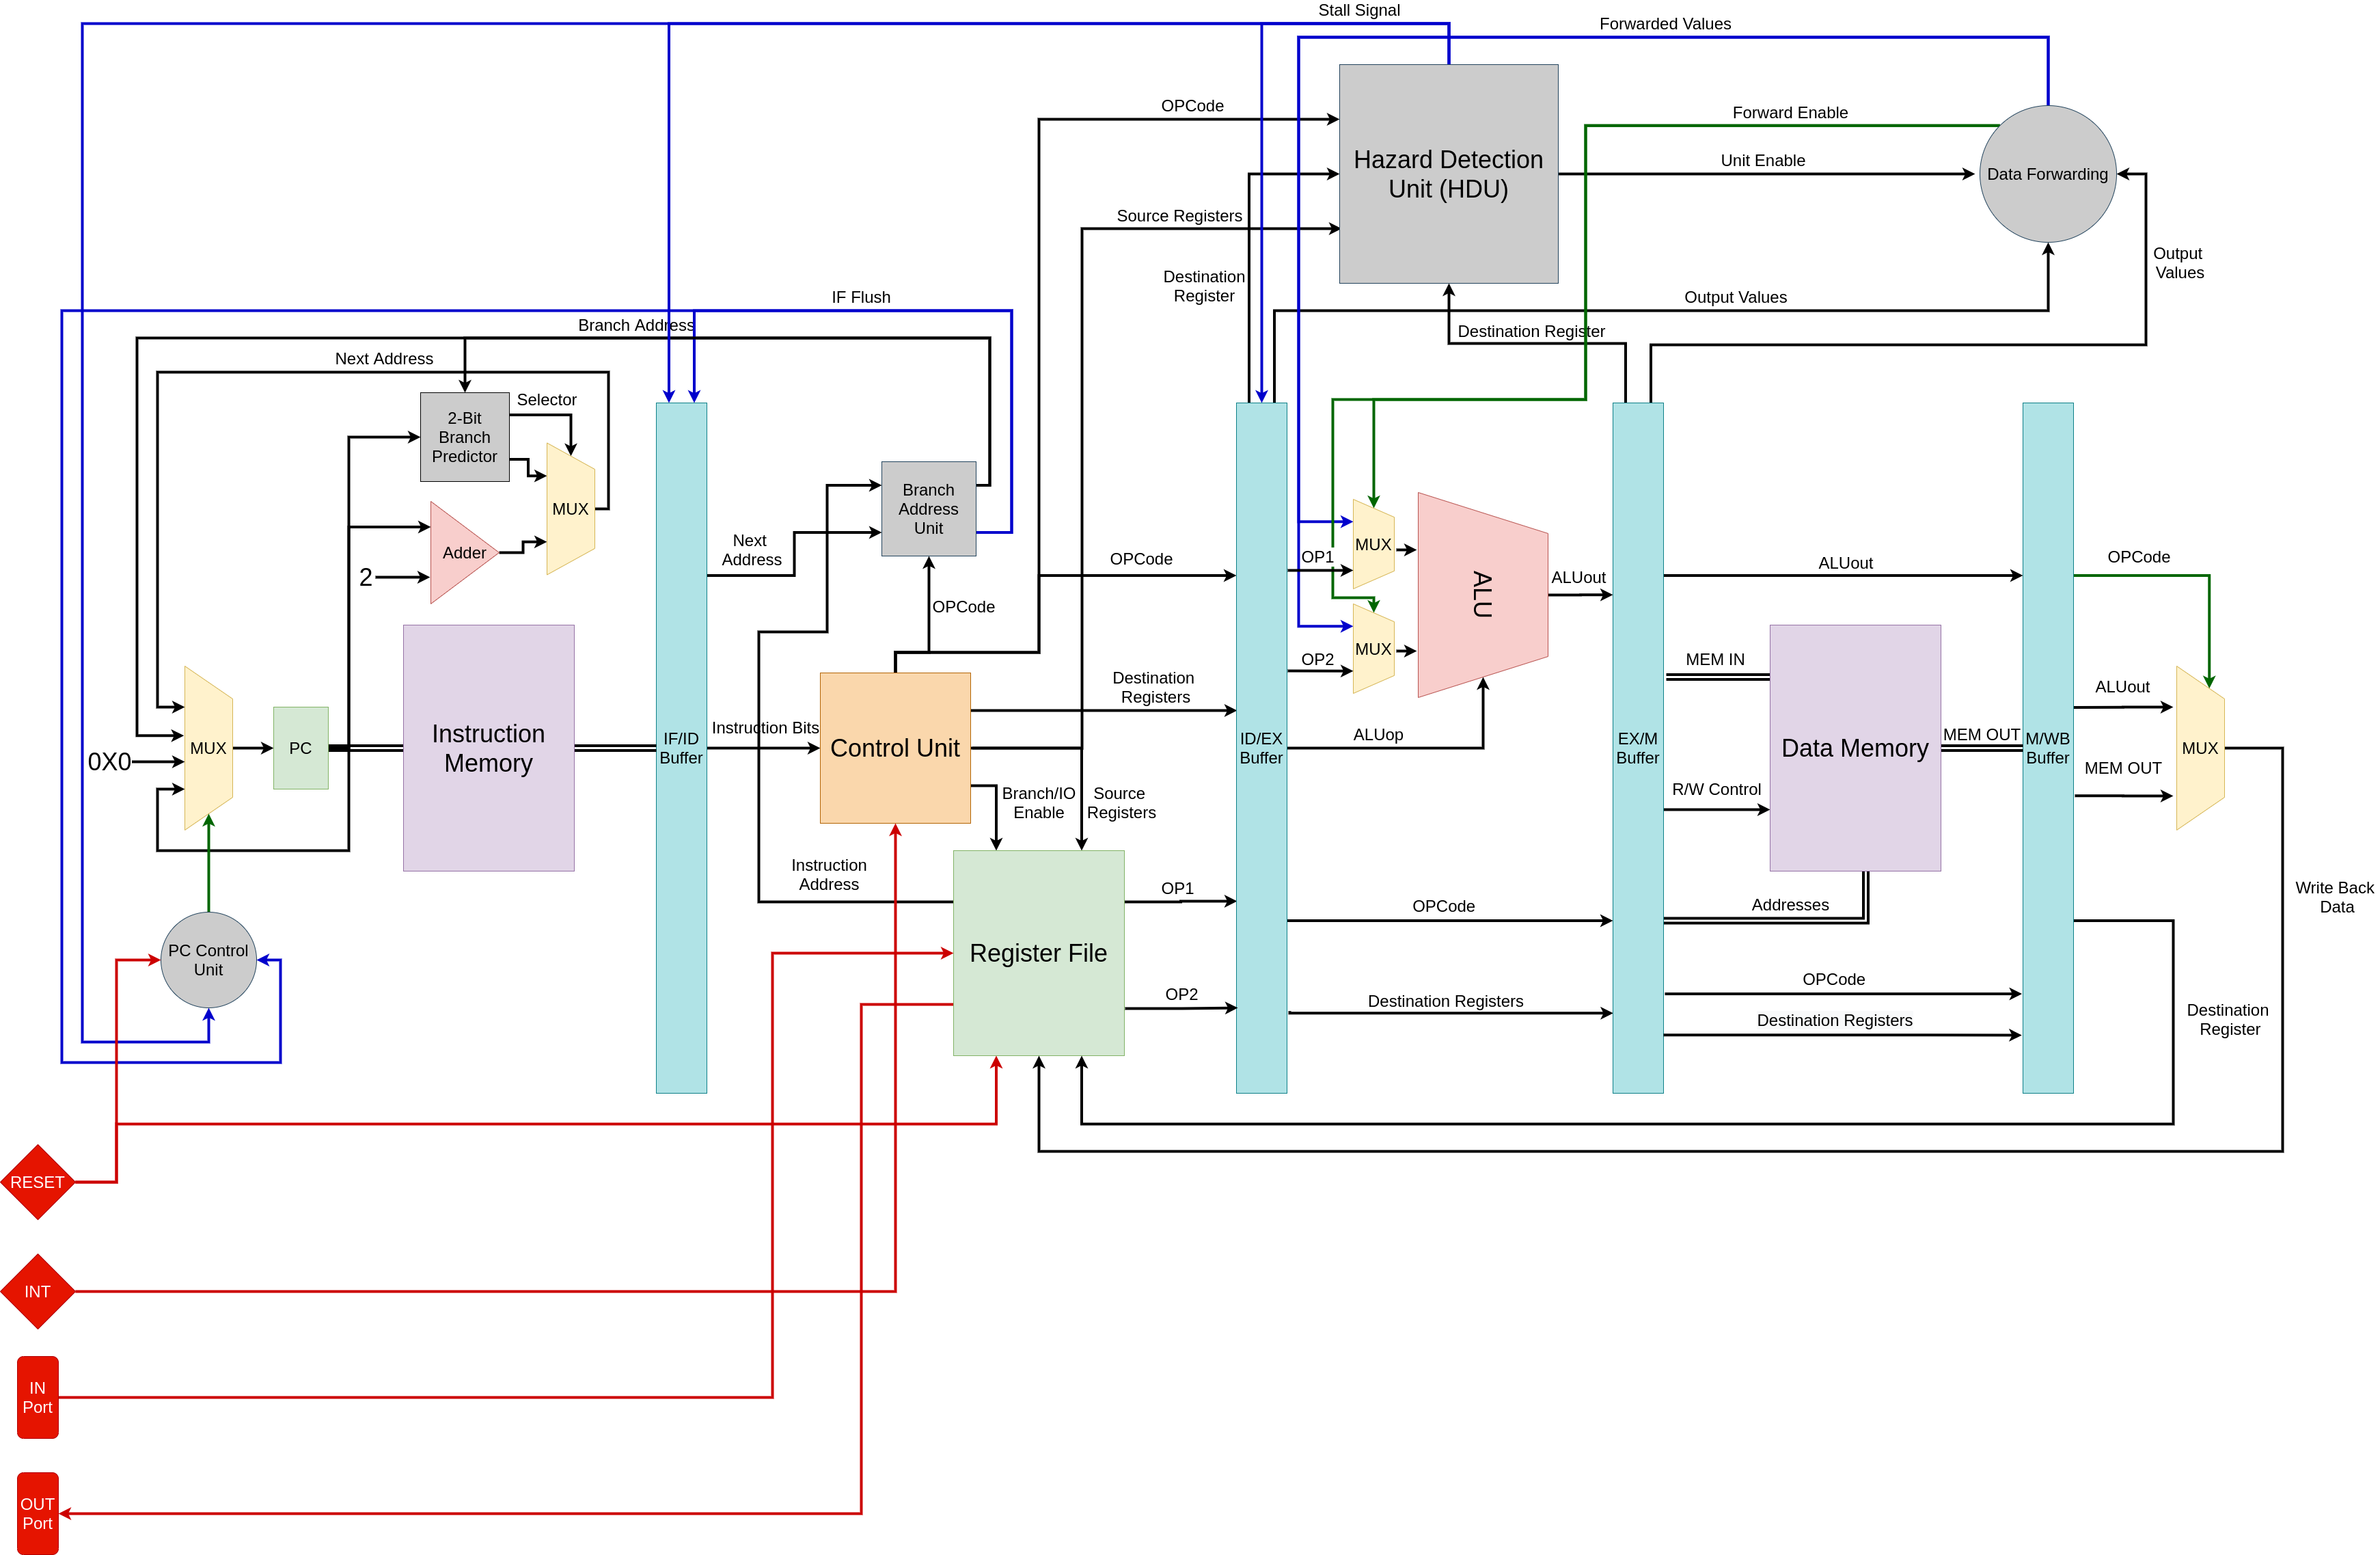
\includegraphics[width=\textwidth]{overall_system}
        \caption{Overall System Design}
        \label{fig:overall}
    \end{figure}
\end{center}
\textbf{TODO(1): Add branch predictor design}\\
\textbf{TODO(2): Add Interrupt handling design}\\
\textbf{TODO(3): Add stack pointer related instructions design}

\section{Memory Specs}
\textbf{TODO: Add both memory specs and figures}

\section{PC Control Unit}
\textbf{TODO: Add PC control unit flow}

\section{Dynamic Branch Prediction}
\textbf{TODO: Add branch prediction details in both overall diagram and section}

\section{Branch Address Unit}
\textbf{TODO: Add branch address unit flow}

\section{Register File}
\textbf{TODO: Add register file flow}

\section{ALU}
\textbf{TODO: Add ALU flow}

\part{Instruction Format}

\section{One Operand Operations}
\begin{itemize}
    \item 4 bits (1111) for one operand instructions.
    \item 3 bits to define instruction.
    \item 3 bits for destination register.
    \item 1 bit to define the memory slots occupied by the instruction.
    \item Total of 11 bits, padded with 5 0's to fit 16 bits.
\end{itemize}
\begin{center}
    \captionof{table}{One Operand Instruction Mapping\label{tab:1op}}
 \begin{tabular}{||c| c| c| c| p{40mm}||} 
 \hline
 Operation & OpCode & Destination & 16$|$32 & Conditions  \\ [0.5ex] 
 \hline\hline
 IN & 1111000 & 000:111 & 0 & ----------------------- \\
 \hline
 NOT & 1111001 & 000:111 & 0 & if !Rdst=0,Z=1 \newline if !Rdst$<$0,N=1 \\
 \hline
 INC & 1111010 & 000:111 & 0 & if Rdst+1=0,Z=1 \newline if Rdst+1$<$0,N=1 \\
 \hline
 DEC & 1111011 & 000:111 & 0 & if Rdst-1=0,Z=1 \newline if Rdst-1$<$0,N=1 \\
 \hline
 OUT & 1111100 & 000:111 & 0 & ----------------------- \\
 \hline
\end{tabular}
\end{center}

\section{Special Operations}
\begin{itemize}
    \item 16 0's to represent NOP (0000000000000000).
\end{itemize}

\section{Two Operand Operations}
\begin{itemize}
    \item 4 bits to define instruction.
    \item 3 bits for each of Rsrc1, Rsrc2 and Rdst.
    \item 1 bit to define the memory slots occupied by the instruction.
    \item 16 bits for immediate values.
    \item Total of 14 bits in most cases with some exceptions mentioned below.
\end{itemize}
\begin{center}
    \captionof{table}{Two Operand Instruction Mapping\label{tab:1op}}
 \begin{tabular}{||c| c| c| c| c| c| c| p{30mm}||} 
 \hline
 Operation & OpCode & Rsrc1 & Rsrc2 & Rdst & imm & 16$|$32 & Conditions  \\ [0.5ex] 
 \hline\hline
 SWAP & 0001 & 000:111 & --- & 000:111 & --- & 0 & ----------------------- \\
 \hline
 ADD & 0010 & 000:111 & 000:111 & 000:111 & --- & 0 & if Result=0,Z=1 \newline if Result$<$0,N=1 \\
 \hline
 SUB & 0011 & 000:111 & 000:111 & 000:111 & --- & 0 & if Result=0,Z=1 \newline if Result$<$0,N=1 \\
 \hline
 AND & 0100 & 000:111 & 000:111 & 000:111 & --- & 0 & if Result=0,Z=1 \newline if Result$<$0,N=1 \\
 \hline
 OR & 0101 & 000:111 & 000:111 & 000:111 & --- & 0 & if Result=0,Z=1 \newline if Result$<$0,N=1 \\
 \hline
 SHL & 0110 & 000:111 & --- & --- & 16 bits & 1 & update carry flag \\
 \hline
 SHR & 0111 & 000:111 & --- & --- & 16 bits & 1 & update carry flag \\
 \hline
 IADD & 1000 & 000:111 & --- & 000:111 & 16 bits & 1 & if Result=0,Z=1 \newline if Result$<$0,N=1 \\
 \hline
\end{tabular}
\end{center}

\section{Memory Operations}
\begin{itemize}
    \item 4 bits to define instruction.
    \item 3 bits for destination register.
    \item 1 bit to define the memory slots occupied by the instruction.
    \item 16 bits for immediate values.
    \item 20 bits for effective addresses.
    \item Total of 8 bits with no immediate values or effective addresses.
    \item Total of 24 bits with immediate values.
    \item Total of 28 bits with effective addresses.
\end{itemize}
\begin{center}
    \captionof{table}{Memory Instruction Mapping\label{tab:1op}}
 \begin{tabular}{||c| c| c| c| c| c| p{40mm}||} 
 \hline
 Operation & OpCode & Rdst & imm & EA & 16$|$32 & Conditions  \\ [0.5ex] 
 \hline\hline
 PUSH & 1001 & 000:111 & --- & --- & 0 & ----------------------- \\
 \hline
 POP & 1010 & 000:111 & --- & --- & 0 & ----------------------- \\
 \hline
 LDM & 1011 & 000:111 & 16 bits & --- & 1 & ----------------------- \\
 \hline
 LDD & 1100 & 000:111 & --- & 20 bits & 1 & ----------------------- \\
 \hline
 STD & 1101 & 000:111 & --- & 20 bits & 1 & ----------------------- \\
 \hline
\end{tabular}
\end{center}

\section{Branch and Change Control Operations}
\begin{itemize}
    \item 4 bits (0000) for branching instructions.
    \item 3 bits to define instruction.
    \item 3 bits for destination register.
    \item 1 bit to define the memory slots occupied by the instruction.
    \item Total of 11 bits, padded with 5 0's to fit 16 bits. 
\end{itemize}
\begin{center}
    \captionof{table}{One Operand Instruction Mapping\label{tab:1op}}
 \begin{tabular}{||c| c| c| c| p{40mm}||} 
 \hline
 Operation & OpCode & Destination & 16$|$32 & Conditions  \\ [0.5ex] 
 \hline\hline
 JZ & 0000001 & 000:111 & 0 & ----------------------- \\
 \hline
 JMP & 0000010 & 000:111 & 0 & ----------------------- \\
 \hline
 CALL & 0000011 & 000:111 & 0 & ----------------------- \\
 \hline
 RET & 0000100 & --- & 0 & ----------------------- \\
 \hline
 RTI & 0000101 & --- & 0 & ----------------------- \\
 \hline
\end{tabular}
\end{center}

\part{Control Signals}
\textbf{TODO: Add related control signals for each instruction}

\part{Pipeline Stages}

\section{Overview}
\textbf{TODO: Add an overview of how pipelining works in our system}

\section{IF/ID Buffer}
\textbf{TODO: Add buffer components}

\section{ID/EX Buffer}
\textbf{TODO: Add buffer components}

\section{EX/M Buffer}
\textbf{TODO: Add buffer components}

\section{M/WB Buffer}
\textbf{TODO: Add buffer components}

\part{Pipeline Hazards and solutions}

\section{Hazards Detection and Handling}
\textbf{TODO: refactor this section and add more details}

\subsection{Structural Hazards}
2 memory units, one for instructions and one for data. Both have the same specs \emph{(mentioned below)}. \\
Also, to handle register file structural hazard, the write back will be in the first half of the clock cycle and the decode will be in the second half.

\subsection{Data Hazards}
Refer the \emph{HDU} in \ref{fig:overall}

\subsubsection{Stall}
Occurs only at Decode stage, due to load use case.
\begin{itemize}
    \item Fetch same instruction (don't increment the program counter).
    \item Latch IF/ID buffer with the same values.
    \item Freeze Decode stage.
    \item Clear ID/EX buffer.
\end{itemize}

\subsubsection{Data Forwarding}
\begin{itemize}
    \item EX/MEM buffer $->$ Execute / Decode.
    \item ID/EX buffer $->$ Decode.
\end{itemize}

\subsection{Control Hazards}
\begin{itemize}
    \item At Fetch stage, always check the branch predictor and calculate the next address accordingly.
    \item At Decode stage, check whether the OPCode is of a branch operation. If so, pass the address to the program counter and compare the correct address with the address of the counter to decide whether to flush the Fetch stage or not. 
\end{itemize}

\subsubsection{Flush}
Occurs only at Fetch Stage, due to wrong branch prediction at Decode stage.
\begin{itemize}
    \item Load new address in the program counter.
    \item Remove fetched instructions from IF/ID buffer.
\end{itemize}

\subsubsection{Dynamic Branch Prediction}
Hash table of some length containing Keys of branch addresses paired with 1-bit for branch prediction.

\end{document}
